\documentclass[../Draft_harmonization_paper.tex]{subfiles}
% \documentclass{article}
% \usepackage[utf8]{inputenc}
% \usepackage{hyperref}
% \usepackage{float}
% \usepackage[table,xcdraw]{xcolor}
% \usepackage{color, colortbl}
% \usepackage{longtable}
% %\usepackage[sort&compress,square,comma,authoryear]{natbib}
% \usepackage{booktabs}
% \usepackage{graphicx}
% \graphicspath{{/home/kunz/Dokumente/Projects/Trait_DB/Invertebrate_traits/Paper/Figures/}}
% \usepackage{longtable}
% \usepackage{rotating}
% \usepackage{geometry}
% \usepackage{array}

% \definecolor{Gray}{gray}{0.9}

% \newcommand{\specialcell}[2][c]{%
%   \begin{tabular}[#1]{@{}c@{}}#2\end{tabular}}

\begin{document}
%! Trait (species) scores along segments of river


\section{Re-analysis of Szöcs et al. 2014 using harmonized and aggregated grouping features}

To investigate how harmonizing grouping features and aggregating invertebrate traits might change the results in the analysis of trait-environment relationships we replicated the data analysis of Szöcs et al. 2014 (\cite{szocs_effects_2014}) using the harmonized grouping features \textit{Body size, Feeding mode, Locomotion, Reproduction/Oviposition, Respiration} and \textit{Voltinism} (21 grouping features have been used in total) and aggregated traits using the aforementioned aggregation methods. The harmonized grouping features used are those that responded strongly to salinity in the study of Szöcs et. al. 2014, except for life cycle duration. %!Aggr. methods
For testing the effect of aggregated traits we assigned to each taxon in Szöcs et al. 2014 the aggregated trait value from the established harmonized European grouping feature database for its corresponding family.

Here, we limit our analysis to the RDA of traits constrained by electric conductivity of the original publication (see appendix \ref{subsec:SI_szoecs_reanalysis} for a more in-depth comparison to the original results). Overall, using the harmonized grouping features lead only to slightly different results in comparison to the original analysis. Sites with high salinity were characterized by multivoltine, ovivoparous, gill-respirating, and shredder species. Only species with the trait life cycle duration $> 1$ year fail to characterize sites with high salinization. Also, life cycle duration $<= 1$ year is not anymore characterizing sites not impacted by salinity. Like in the original analysis, transition and upstream sites from the point source are characterized by univoltine species and species that lay their eggs in an aquatic environment. The usage of aggregated traits yielded similar species scores for every aggregation method. Also, for every aggregation method compared, using at family-level aggregated traits did only slightly change the RDA species scores compared to not aggregated traits (Figure \ref{fig:rda_species_scores}). Hence, the interpretation of the trait composition is the same as when only using harmonized grouping features. An overview of the harmonization for the European trait databases can be found in the supporting information in section \ref{sec:SI_harmonization_EU}.

% Mention that threshold according to mahalanobis distance is almost reached for life cycle duration

% Species scores
\begin{figure}[H]
    \label{fig:rda_species_scores}
    \centering
    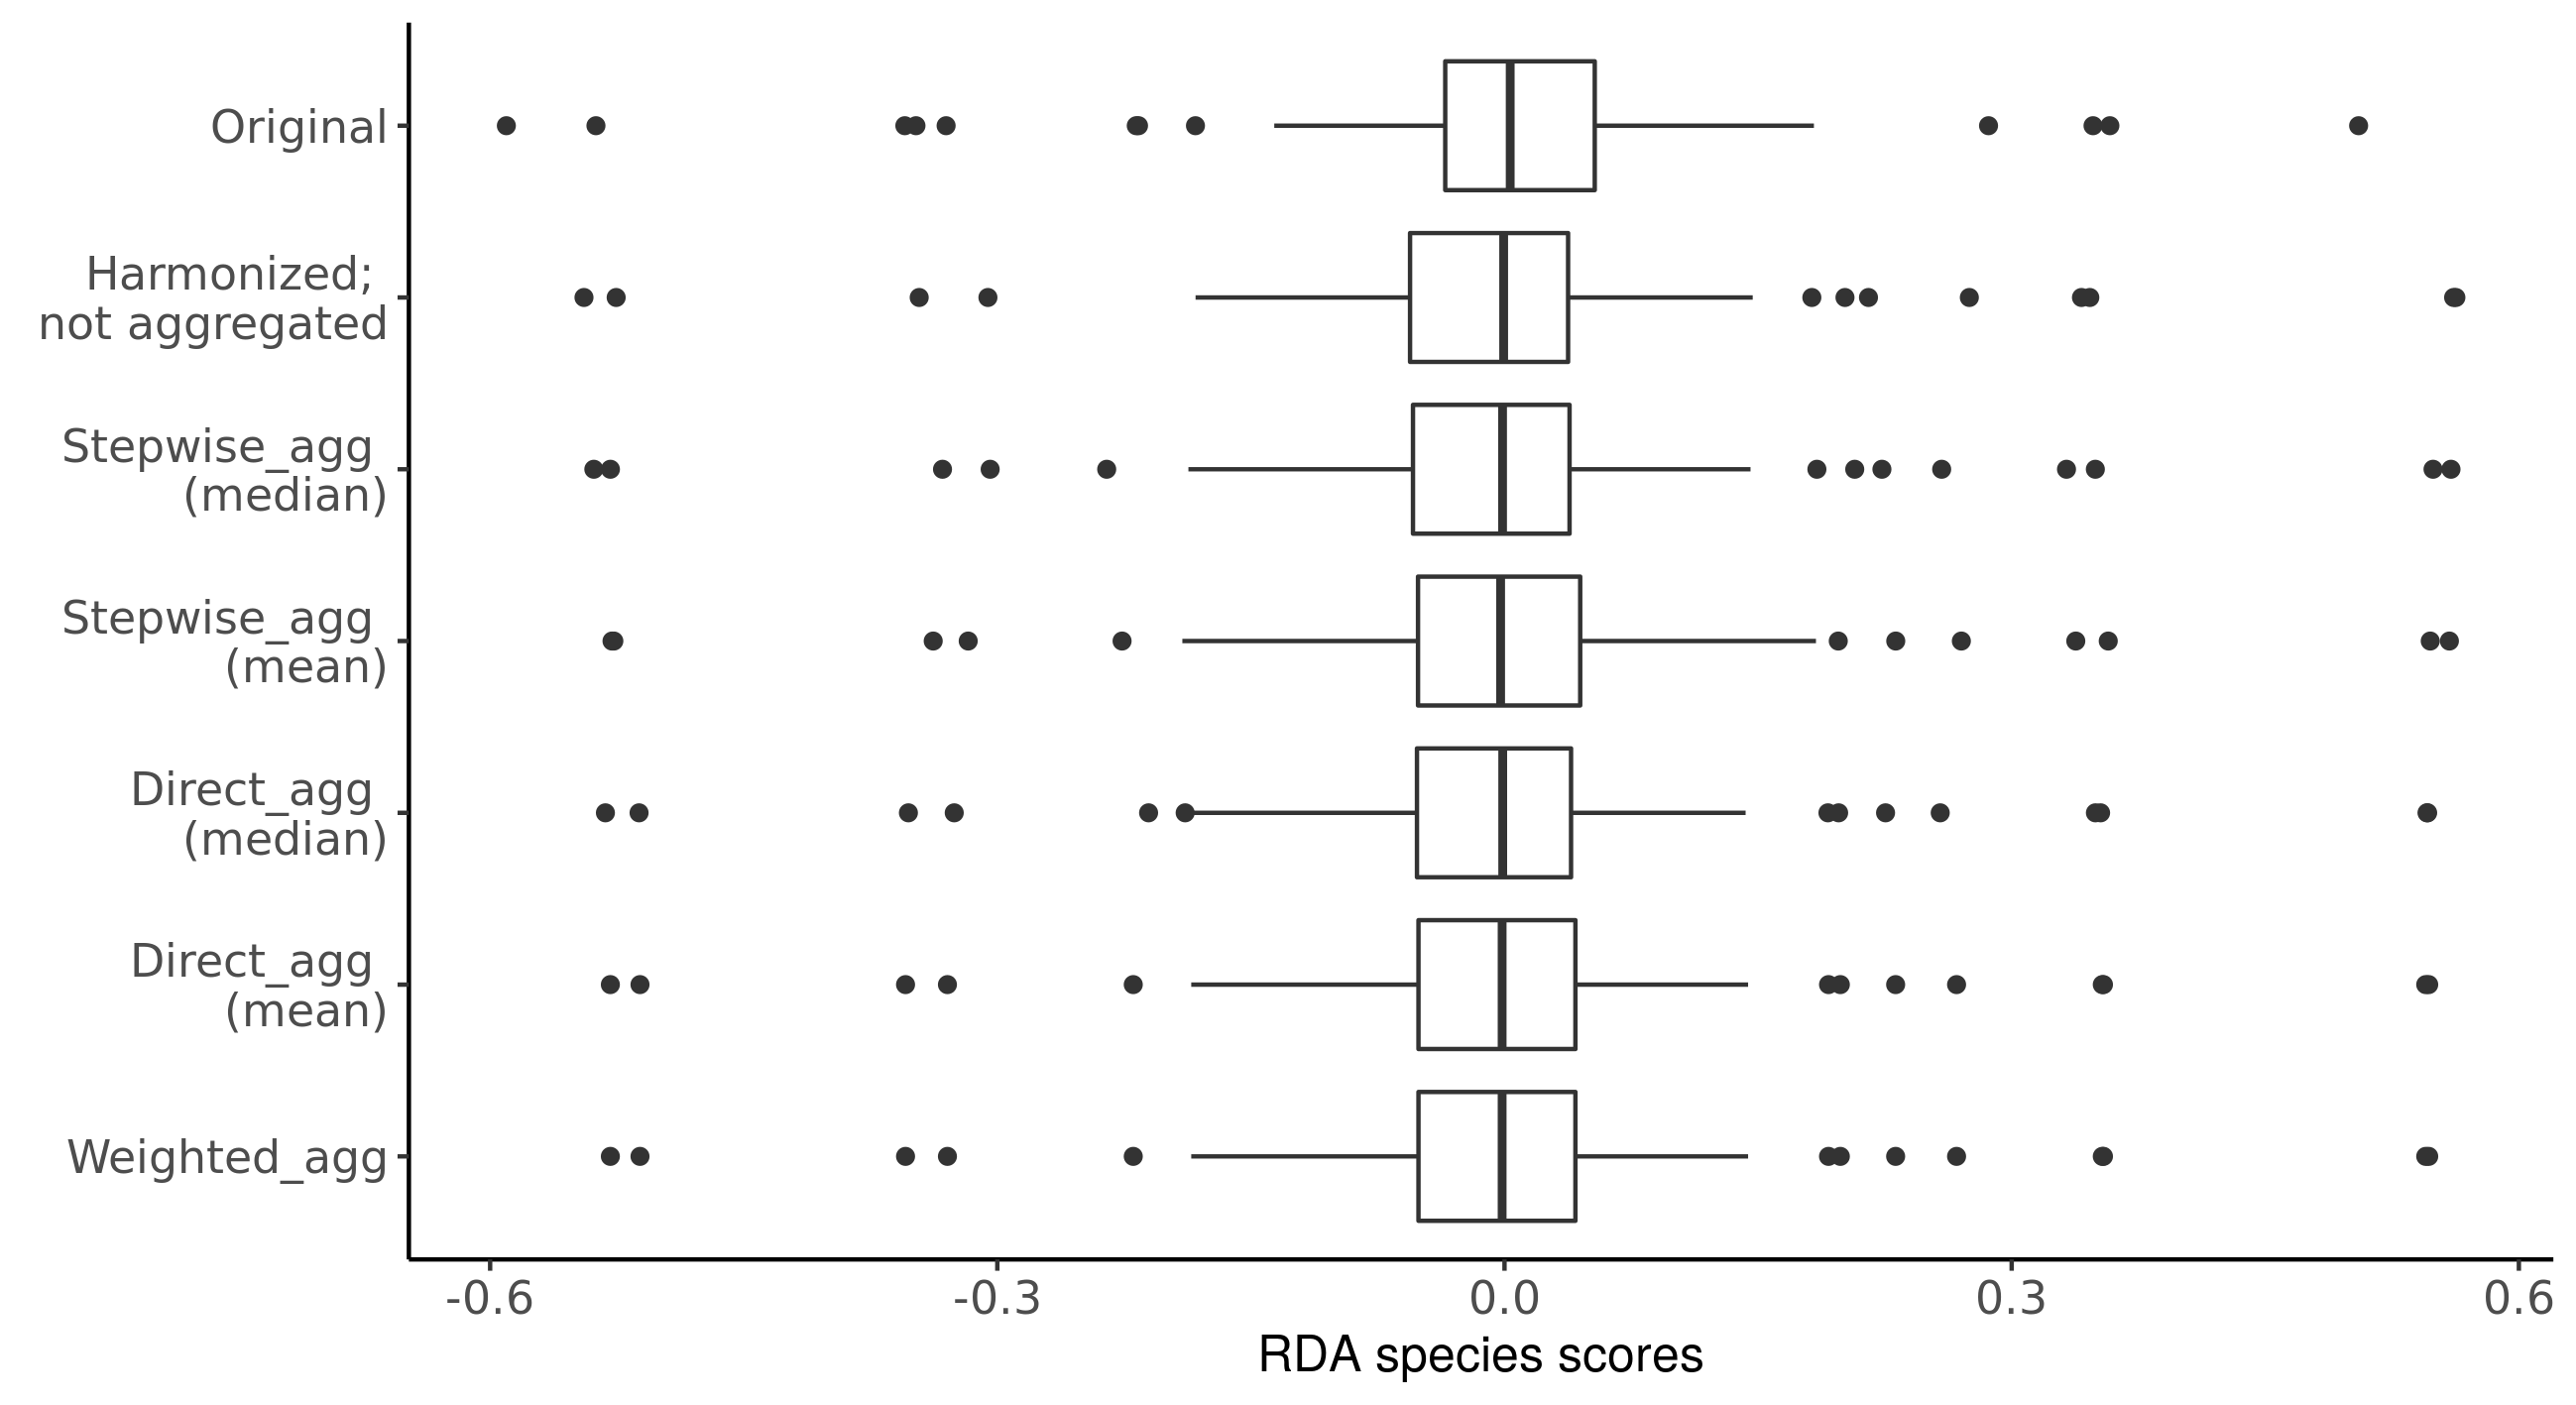
\includegraphics[width=16.5cm, height=10cm]{Species_scores_rda.png}
    \caption{Species scores obtained by RDA from the original analysis (\cite{szocs_effects_2014}), using harmonized grouping features, and using harmonized grouping features with assigned trait affinities from traits aggregated to family-level.}
    \label{fig:rda_species_scores}
\end{figure}

\end{document}